\documentclass[style=upen, size=14pt]{powerdot}
\usepackage{natbib}
\usepackage{bibentry}
\definecolor{arany}{RGB}{255,242,0}
\hypersetup{backref=page}
\hypersetup{
  colorlinks=true,
  citecolor=cyan,
  linkcolor=cyan,
  filecolor=magenta,      
  urlcolor=cyan}
\usepackage{graphicx}
\usepackage{amsmath}
\DeclareMathOperator*{\argmax}{argmax}
\DeclareMathOperator*{\argmin}{argmin}
\usepackage{amssymb}
\usepackage{stmaryrd}
\usepackage[latin2]{inputenc}
%\usepackage[magyar]{babel}
%\usepackage{euler}
\usepackage{tikz}
\usepackage{tikz-qtree}
\usepackage{tikz-dependency}
\usepackage{linguex}
\usepackage{amsthm}

\tikzset{every tree node/.style={align=center,anchor=north}}
%\usepackage{tabularx}
%\usepackage{threeparttable}
%\usepackage{color}
%\selectlanguage{english}
%\frenchspacing
\newcommand{\nd}{\noindent}
\newcommand{\Val}{\mathop{\mathit{Val}}}
\newcommand{\gold}{\color{arany}}
%\usepackage{tikz}
%\usepackage{tikz-qtree}
%\newcommand{\qed}{\hfill\mbox{\raggedright \rule{.1in}{.1in}}}
\def\es{\mathbin\land}
\theoremstyle{definition}
\newtheorem*{definition}{Definition}
\newtheorem{axioma}{Axiom}
\newtheorem{tetel}{Theorem}
\newtheorem{prop}{Proposition}
\newtheorem{lemma}{Lemma}
\begin{document}

\title{Natural Language Processing\\~~\\Lecture 3\\Tokenization}
% \author{}

\date{2021}
\maketitle

\begin{slide}[toc=Whitespace splitting]{Baseline: splitting on whitespace}
  For many writing systems, splitting the text at \emph{white spaces} is a
  useful baseline:\bigskip

  'This isn't an easy sentence to tokenize!' $\Rightarrow$ \\
  
  ['This', "isn't", 'an', 'easy', 'sentence', 'to', 'tokenize!']\bigskip

  Problems:
  \begin{itemize}
  \item we typically want to treat punctuation marks as separate tokens (but
    only if they are really punctuation, think of 'U.K.' or '10,000.00\$'); 
  \item this solution cannot separate token pairs without white space between
    them, e.g.,  expressions with clitics like "isn't".
  \end{itemize}
\end{slide}

\begin{slide}[toc=Regular expressions]{Regular expressions}
  We need to introduce more sophisticated patterns to describe token boundaries
  in context-dependent way. A popular solution is using \emph{\gold regular
    expressions} (regexes for short).\bigskip

  Given a finite $\Sigma$ alphabet of symbols, regexes over $\Sigma$ and their
  matches in $\Sigma^*$ are defined by simultaneous recursion as follows:
  \begin{enumerate} 
  \item The empty string and any single symbol in $\Sigma$ is a regex
    over $\Sigma$ and matches itself.
  \end{enumerate}
\end{slide}

\begin{slide}[toc=]{Regular expressions cont.}
  \begin{enumerate}
     \setcounter{enumi}{1}
  \item If $r_1$ and $r_2$ are regexes over $\Sigma$ then
    \begin{enumerate}
    \item their \emph{\gold concatenation}, $r_1 r_2$ is also a regex over $\Sigma$ and
      matches exactly those strings that are the concatenation of a string
      matching $r_1$ and a string matching $r_2$, and
    \item their \emph{\gold alternation}, $r_1 \vert r_2$ is also a regex over
      $\Sigma$ and matches exactly those strings that match either $r_1$ or
      $r_2$.
    \end{enumerate}
  \item If $r$ is a regex over $\Sigma$ then applying the \emph{\gold Kleene
      star} operator to $r$ we can form a new regex $r^*$ which matches exactly
    those strings that are the concatenation of 0 or more strings each
    matching $r$.
  \end{enumerate}
\end{slide}

\begin{slide}[toc=]{Formal languages}
  Given a finite alphabet $\Sigma$, a \textit{formal language} $\mathcal L$
  is an arbitrary set of strings over $\Sigma$. These strings are often
  defined via a \textit{grammar}. \medskip

  Based on the complexity of the grammar, languages can be classified into
  different \textit{types}. The most well-known is the Chomsky hierarchy:

  \begin{center}
    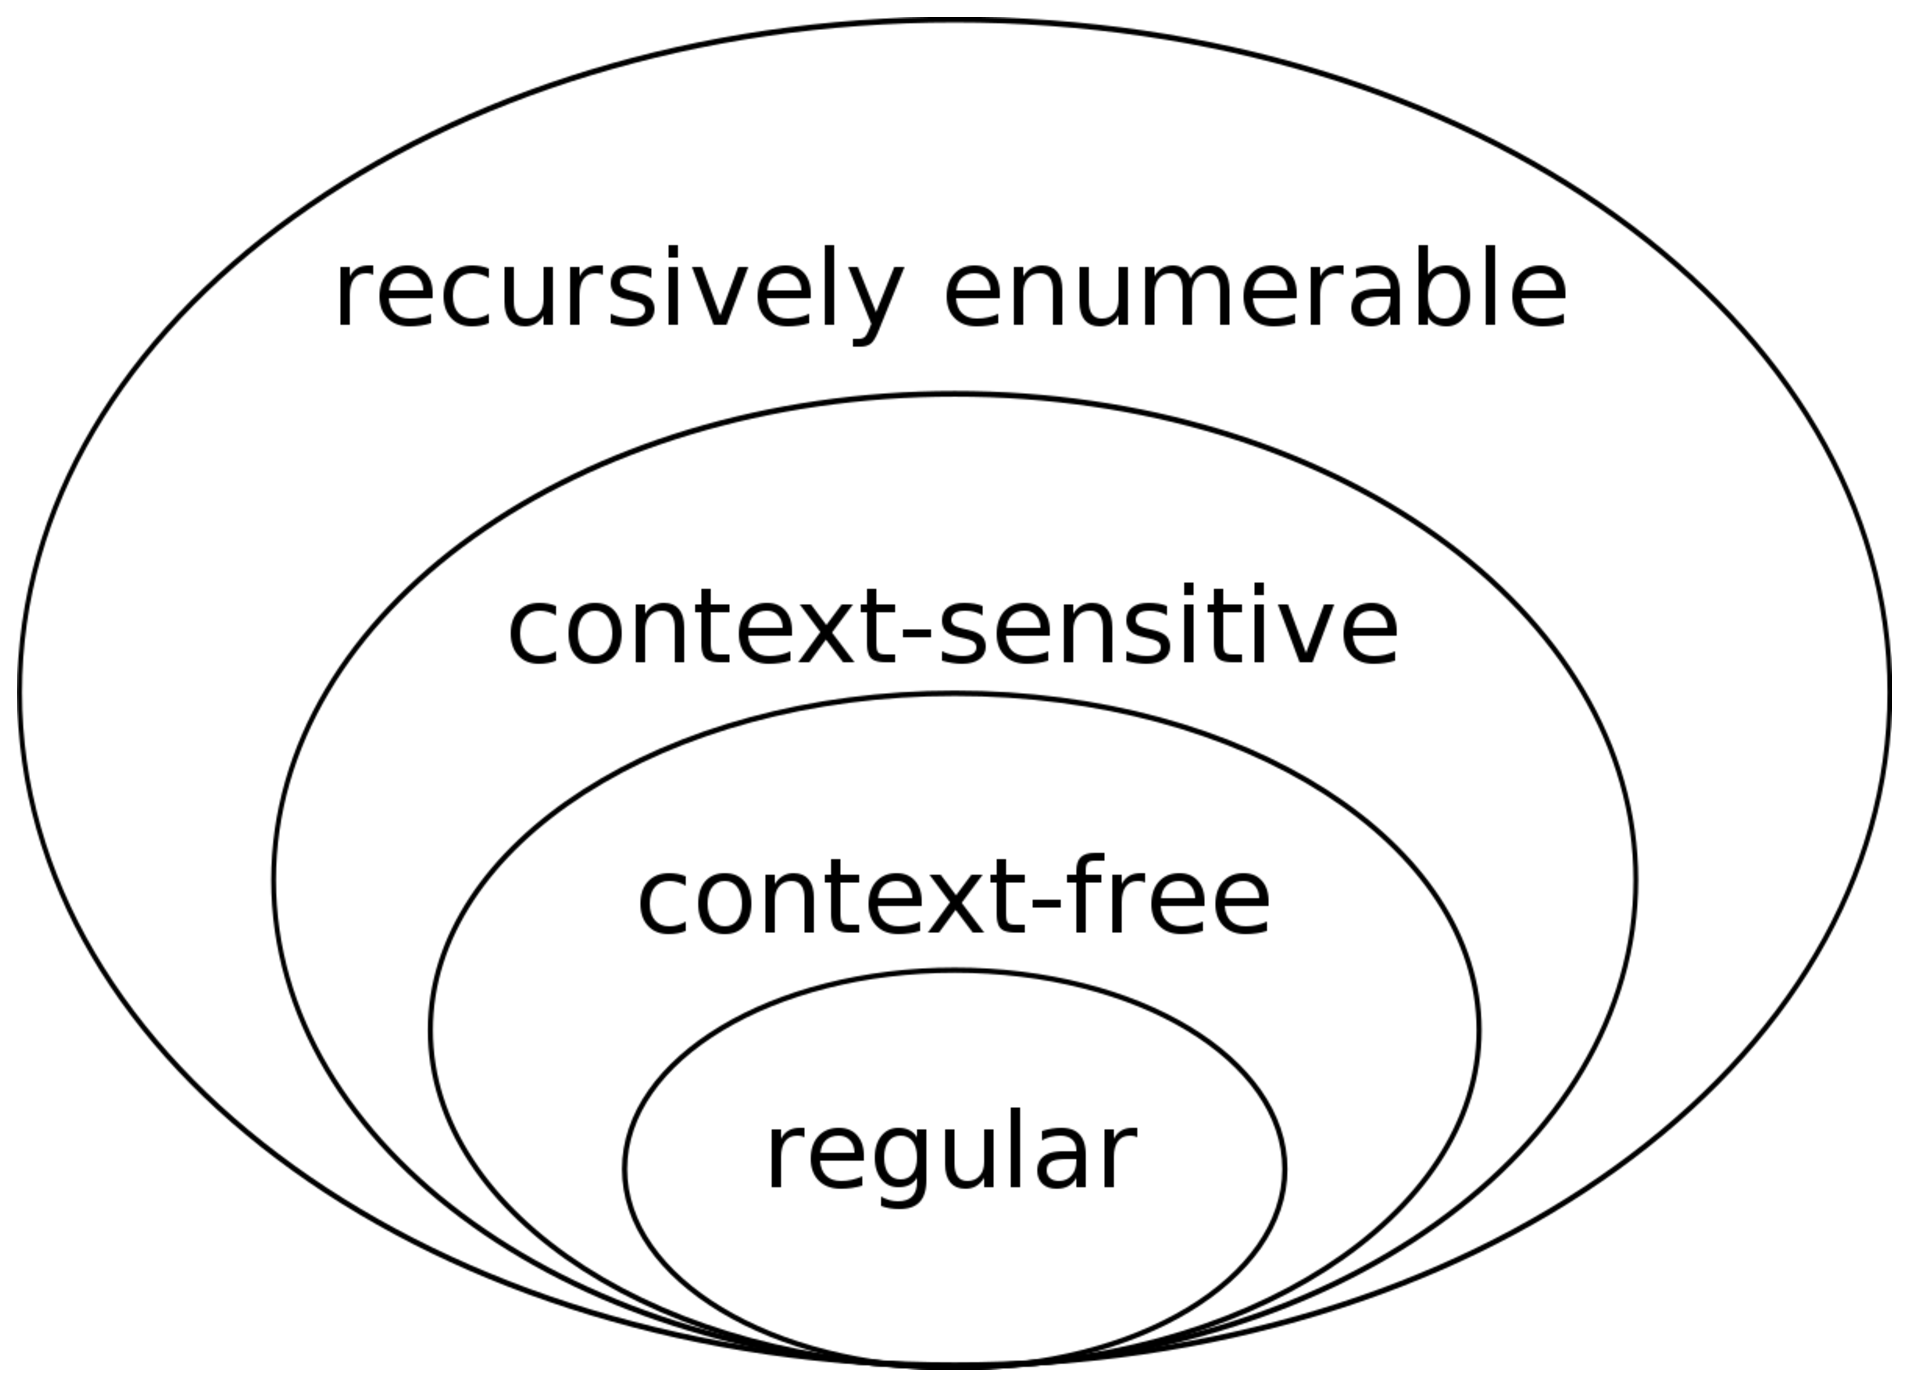
\includegraphics[width=0.4\textwidth]{figures/chomsky_hierarchy.eps}

    \footnotesize{(Figure from \href{https://en.wikipedia.org/wiki/Chomsky_hierarchy}{Wikipedia})}
  \end{center}
\end{slide}

\begin{slide}[toc=]{Formal languages cont.}
  \begin{itemize}
    \item Regular languages: can describe linear structures
      \begin{itemize}
        \item Programming: state machines
        \item Languages: words, noun phrases
      \end{itemize}
    \item Context-free languages: can describe tree structures
      \begin{itemize}
        \item Programming: XML DOM, parse trees
        \item Languages: phrase structure grammars (of sentences)
      \end{itemize}
    \item Context sensitive languages: most human languages are mildly context
      sensitive
    \item Recursively enumerable: all problems that can be solved by an
      algorithm
  \end{itemize}
\end{slide}

\begin{slide}[toc=]{Back to regular expressions...}
  A formal language $\mathcal L$ is \emph{\gold regular} iff there exists a
  regular expression that matches exactly $\mathcal L$'s elements.\bigskip

  There are simple formal languages that are not regular, e.g., the ``twin
  language'' $\{ww ~\vert~ w \in \{a, b\}^* \}$.\bigskip

  Nonetheless, regular expressions are flexible enough for a lot of practical
  tasks, and there are higly efficient algorithms for deciding whether an $s$
  string matches a regex (with $\mathcal O(\mathrm{length}(s))$ time
  complexity).
\end{slide}

\begin{slide}[toc=]{Regular languages and FS acceptors}
  Finite state acceptors are finite state machines that consume an input
  sequence of characters and can "accept" or "reject" the input. They differ
  from the simplest possible FSA-s by having
  \begin{itemize}
  \item an explicit \emph{\gold start state},
  \item a set of designated \emph{\gold accepting states}, and
  \item their transitions labeled with symbols from a finite alphabet, or with
    the empty string.
  \end{itemize}
  An FS acceptor \emph{\gold accepts} an input iff it has a sequence of
  transitions which starts from the start state, ends in an accepting state, and
  the concatenation of the transition labels is the input in question.
\end{slide}

\begin{slide}[toc=]{Regular languages and FS acceptors cont.}
  An acceptor for the words "car", "cars", "cat" and "cats".
  \begin{center}
    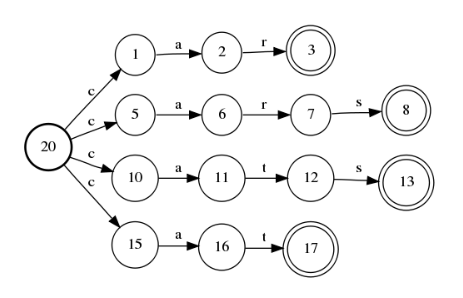
\includegraphics[width=0.6\textwidth]{figures/fsa1.eps}
  \end{center}
  Can be simplified to (figures from \cite{buutbogel2009fsmorph}):
  \begin{center}
    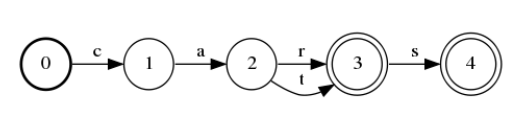
\includegraphics[width=0.6\textwidth]{figures/fsa2.eps}
  \end{center}
\end{slide}

\begin{slide}[toc=]{Regular languages and FS acceptors cont.}
  The connection between FS acceptors and regular languages/expressions is
  established by Kleene's \emph{\gold Equivalence Theorem}:
  \begin{itemize}
  \item A language is regular iff there is an FSA acceptor that accepts exactly
    its elements.\footnote{See, e.g.,
      \href{https://bit.ly/2ZHlKWG}{https://bit.ly/2ZHlKWG} for a proof.}
  \end{itemize}
  This equivalence is important both theoretically and practically: there are
  very efficient algorithms to simplify/minimize FS acceptors and also to decide
  whether they accept a string or not.
\end{slide}

\begin{slide}[toc=]{Regular expressions: extensions}
  \emph{\gold Convenience extensions} not increasing expressive power just adding useful
  shortcuts, e.g.;
  \begin{itemize}
  \item character classes matching any single symbol in a set, e.g. [0-9];
  \item complemented character classes matching any character \emph{not} in the
    complemented set, e.g. [\^{}ab];
  \item operators for specifying the required number of pattern repetitions,
    e.g., $r\{m,n\}$ matches $s$ if $s$ repeats the $r$ pattern $k$ times, with
    $m\leq k \leq n$.
  \item optional matching: $r? = r\{0,1\}$
  \item Kleene plus: $r+ \approx r\{1,\infty\}$
  \end{itemize}
\end{slide}

\begin{slide}[toc=]{Regular expressions: back-references}
  So-called \emph{\gold back-reference} constructions, in contrast, that allow
  naming and referencing match(es) corresponding to earlier parts of the regex
  \emph{increase} the expressive power.\bigskip

  For example, most current regex libraries allow a regex similar to\bigskip

  \begin{center}
    (?P$<$a$>$[ab]*)(?P=a)\bigskip
  \end{center}

  which uses back-reference to define exactly the aforementioned non-regular
  ``twin language''.
\end{slide}

\begin{slide}[toc=]{Regex-based find and replace}
  In addition to matching whole strings against a regex, two regex-based tasks are
  very common:
  \begin{itemize}
  \item finding substrings of a string that match a regex,
  \item regex-based find-and-replace: in its simplest form this is replacing
    matching substrings with a given string, but two notable
    extras are provided by modern regex libraries:
    \begin{itemize}
    \item the regex can have look-ahead and look-back parts, that are used when
      finding a match but do not count in the part which is replaced;
    \item replacements do not have to be fix -- they can contain back-references
      to parts of the match.
    \end{itemize}
  \end{itemize}
\end{slide}

\begin{slide}[toc=Regex cascade]{Regex cascade-based tokenization}
  Core idea: perform regex-based substitutions on the input so that in the end
  it's enough to split on white spaces.\bigskip

  The
  \href{ftp://ftp.cis.upenn.edu/pub/treebank/public_html/tokenizer.sed}{tokenizer
    sed script} accompanying the Penn Tree Bank is a good example. A few
  representative rules (\textbackslash \& refers back to the full match,
  \textbackslash $n$ to the $n$-th group):\bigskip

  '...' $\Rightarrow$ ' ... ' (separate ellipsis)
  
  '[,;:\#\$\%\&]' $\Rightarrow$ ' \textbackslash \& ' (separate various signs)

%   # Assume sentence tokenization has been done first, so split FINAL periods
%   # only.
  
  ([\^{}.]){(}[.]){\Large(}{\large[}]){\small\}}"'{\large]}*{\Large)}[\quad]*\$ $\Rightarrow$ '\textbackslash 1 \textbackslash 2\textbackslash 3'

  (assume sentence input and split FINAL periods only)

  "'ll" $\Rightarrow$ " 'll" (separate clitic 'll)
\end{slide}

\begin{slide}[toc=]{Regex cascade-based tokenization cont.}
  The main problem for the approach is the proper handling of exceptions: e.g.,
  word ending periods should be split, \emph{except for abbreviations}.\bigskip

  The standard solution is to replace the problematic expressions with
  unproblematic placeholders before executing the substitutions in question, e.g.\smallskip

  \begin{center}
    (etc\textbackslash.$\vert$i\textbackslash.e\textbackslash.$\vert$e\textbackslash.g\textbackslash.)
    $\Rightarrow$ $<$abbrev$>$
  \end{center}\smallskip
  
  This solution requires keeping track of the placeholder substitutions and
  restoring the originals after executing the problematic rules.
\end{slide}

\begin{slide}[toc=Lexers]{Lexer-based solutions}
  They use off-the shelf ``lexers'' (lexical analyzers), originally developed
  for the tokenization/lexical analysis of computer programs.

  A typical lexer takes a character stream as input and produces a stream of
  classified tokens from it:

  \begin{center}
    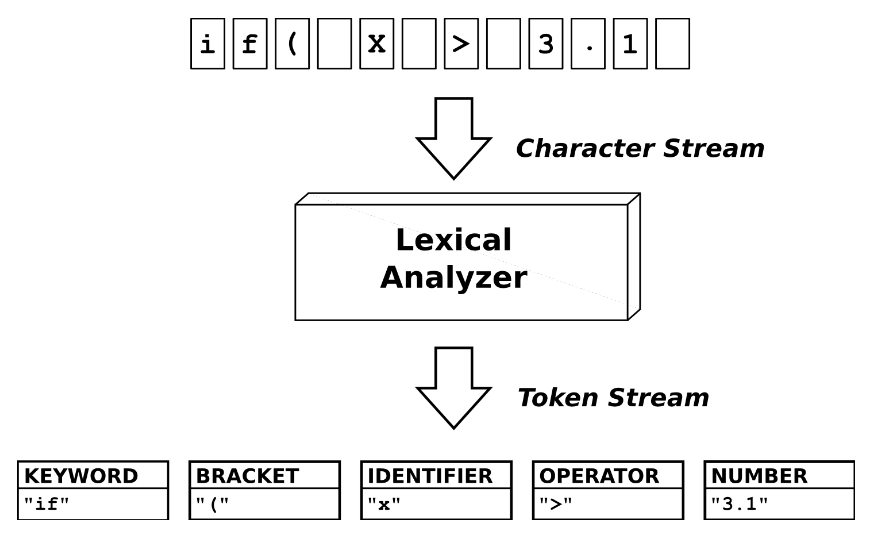
\includegraphics[width=0.6\textwidth]{figures/lexer.eps}
  \end{center}
\end{slide}

\begin{slide}[toc=]{Lexer-based solutions cont.}
  Most lexers are actually lexical analyser generators. Their input is a list of
  token classes (types), regular expression patterns and\smallskip

  \begin{center}
    [\textsc{RegexPattern}] $\Rightarrow$ [\textsc{Action}]\smallskip
  \end{center}

rules (where the most important action is classifying the actual match as a
token of a given type), and they generate a concrete, optimized lexical analyzer
implementing the given rules, e.g., by generating the C source code of the
analyzer.
\end{slide}

\begin{slide}[toc=spaCy]{Case study: spaCy's rule-based tokenizer}
  % To appreciate how a purpose-built, rule-based NLP tokenizer might look like,
  % let's look briefly at spaCy's built in tokenizer. The following explanation is
  % from the spaCy website's tokenization section:

  \begin{enumerate}
  \item The input text is split on white space.\footnote{The algorithm
    description is from the
    \href{https://spacy.io/usage/linguistic-features\#tokenization}{spaCy
      documentation.}}
  \item Then, the tokenizer processes the text from left to right. On each
    substring, it performs two checks:
    \begin{enumerate}
    \item Does the substring match a tokenizer exception rule? For example,
      "don't" does not contain whitespace, but should be split.
    \item Can a prefix, suffix or infix be split off? For example punctuation
      like commas, periods.
    \end{enumerate}
    If there's a match, the rule is applied and the tokenizer continues
    its loop, starting with the newly split substrings.
  \end{enumerate}

\end{slide}

\begin{slide}[toc=]{SpaCy's rule-based tokenizer cont.}
  A simple example: tokenizing \emph{``Let's go to N.Y.!''}
    \begin{center}
      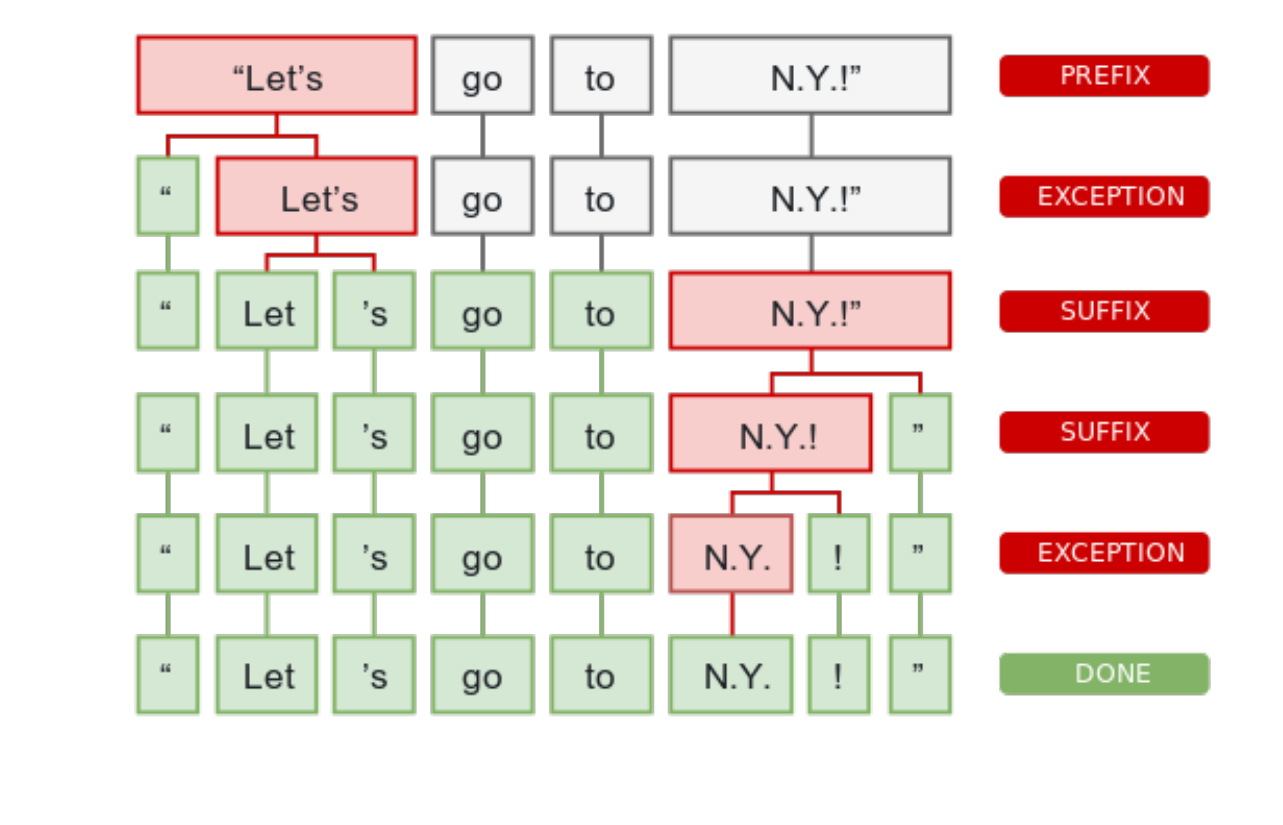
\includegraphics[width=0.9\textwidth]{figures/spacy_tokenizer.eps}\
      
      \footnotesize{(Figure from the \href{https://spacy.io/usage/linguistic-features\#tokenization}{spaCy documentation})}
    \end{center}
\end{slide}

\begin{slide}[toc=Edit distance]{Edit distance}
  In addition to segmenting the input into units, tokenization also involves
  classifying tokens into types, deciding e.g., which type(s)\smallskip
  \begin{center}
    'Apple', 'apple', 'appple'\smallskip
  \end{center}
  belong to. In many cases, these decisions require a \emph{similarity metric}
  between strings.

  One of the most important metric families in this domain is the so-called
  \emph{\gold edit distance} family, which measures the distance between two
  strings by the minimal number of edit operations required to transform them
  into each other.
\end{slide}

\begin{slide}[toc=]{Edit distance cont.}
  Given
  \begin{itemize}
  \item a set of \emph{\gold editing operations} (e.g., removing or inserting a character
    from/into the string) and
  \item a \emph{\gold weight function} that assigns a weight to each operation,
  \end{itemize}
  the \emph{\gold edit distance} between two strings, a source and a target, is
  the minimum total weight that is needed for transforming the source into the
  target.
\end{slide}
    
\begin{slide}[toc=]{Levenshtein distance}
  One of the most important variants is the so-called Levenshtein distance,
  where the operations are the
   \begin{itemize}
  \item deletion,
  \item insertion, and
  \item substitution of a character,
  \end{itemize}
  and the weight of all operations is 1.0.
  \begin{center}
    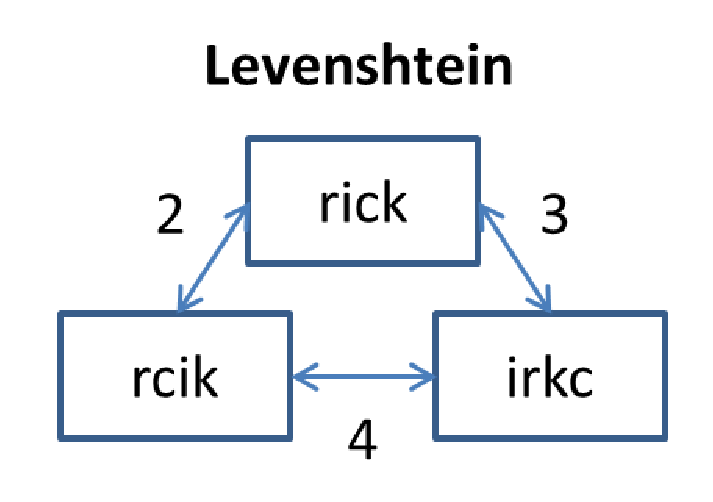
\includegraphics[width=0.4\textwidth]{figures/levenshtein.eps}\
    
    \footnotesize{(Figure from \href{https://devopedia.org/levenshtein-distance}{Devopedia})}
  \end{center}
\end{slide}


\begin{slide}[toc=Subword tokenization]{Tokenization vs subword tokenization}
  Classical tokenization aims at segmenting the input character stream precisely
  into linguistically motivated units: words and punctuation.

  This type of
  tokenization is useful for human linguistic analysis, but not for building
  large language models: it

  \begin{itemize}
  \item is rather challenging, because there is a wide variety of writing systems
    and languages that all require (sometimes radically) different rules/models;
  \item generates huge vocabularies on larger corpora, and still leads to
    problems with out of vocabulary words.
  \end{itemize}
\end{slide}

\begin{slide}[toc=]{Tokenization vs subword tokenization cont.}
  A recently developed alternative is \emph{subword tokenization}.

  A large number of modern deep, end-to-end NLP architectures use
  subword-tokenization instead of classical tokenization for segmenting the
  input.\bigskip

  The main advantages are
  \begin{itemize}
  \item requires no or only very minimal pretokenization;
  \item statistical and data-driven: learns the segmentation model from a corpus
        (no manual rule writing);
  \item vocabulary size can be freely chosen; it will contain the most frequent
        word and subword units;
  \item writing and language-agnostic;
  \end{itemize}
\end{slide}

\begin{slide}[toc=]{Tokenization vs subword tokenization cont.}
  What this means for the text:
  \begin{itemize}
  \item the input text will be segmented into the most frequent words and
        subwords
  \item quality of the segmentation depends on the vocabulary size,
      \begin{itemize}
      \item for a single language, 30,000 types is enough
      \item a regular vocabulary is in the hundred thousands or even millions
      \end{itemize}
  \item \textit{no out-of-vocabulary words} (with the right settings!),
  \item the subword segments are in usually informative, boundaries are
        frequently close to morphological ones.
  \end{itemize}
\end{slide}

\begin{slide}[toc=Byte Pair Encoding]{Byte Pair Encoding (BPE)}
  BPE was originally a simple compression technique for byte sequences, but can
  be generalized to any sequence consisting of symbols from a finite alphabet.
  To generate an encoded / compressed version of a sequence over an alphabet,
  \begin{enumerate}
  \item initialize the symbol list with the symbols in the alphabet, and
  \item repeatedly count all symbol pairs and replace each occurrence of the
    most frequent pair ('A', 'B') with a new 'AB' element, and add 'AB' to the
    list of symbols.
  \end{enumerate}
\end{slide}
    
\begin{slide}[toc=]{Byte Pair Encoding (BPE) cont.}
  How can this technique be used for subword tokenization of texts? The trick is
  to learn the vocabulary used for segmentation from a training corpus by
  applying BPE to the text. Modifications to basic BPE:
  \begin{itemize}
  \item start with a rough pretokenization into words (frequently highly simple,
    e.g. split on white space),
  \item do not allow BPE merges to cross word boundaries.
  \end{itemize}
  In practice these modifications are frequently implemented by adding a new
  '\_' word-end (or word-start) symbol to the alphabet, and stipulating that
  '\_' can only end (or start) merged items.
\end{slide}

\begin{slide}[toc=]{Byte Pair Encoding (BPE) cont.}
  A simple example: BPE encoded versions of a sentence after different numbers
  of merge operations.
  \begin{center}
    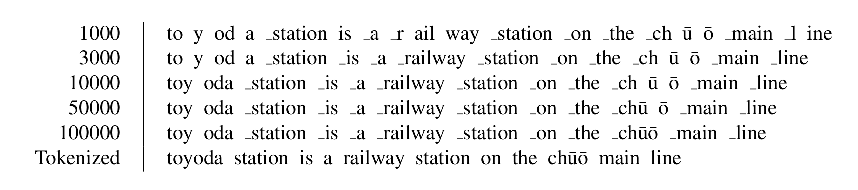
\includegraphics[width=1.\textwidth]{figures/bpe.eps}
    \footnotesize(Table from \href{http://www.lrec-conf.org/proceedings/lrec2018/pdf/1049.pdf}{BPEmb: Tokenization-free Pre-trained Subword Embeddings})
  \end{center}
  As the number of merges increases, more and more symbols are full words.
\end{slide}

\begin{slide}[toc=]{Greedy BPE subword tokenization}
  Processing a corpus with BPE results in a 'vocabulary' of all characters
  together with the results of all merges. New pretokenized input is then
  subword tokenized by greedily matching the words against this
  vocabulary/dictionary from left to right:

  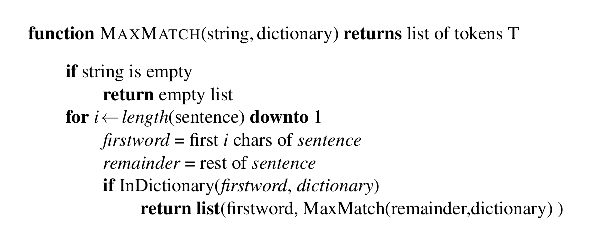
\includegraphics[width=1.\textwidth]{figures/max_match.eps}
  
  \footnotesize(From \href{https://web.stanford.edu/~jurafsky/slp3/2.pdf}{ch. 2 of Jurafsky and Martin's \emph{Speech and Language
      Processing} (3rd ed.)})

  \end{slide}

\begin{slide}[toc=WordPiece]{WordPiece}
  WordPiece is another subword tokenization method that is only slightly
  different from BPE. The differences are:
  \begin{itemize}
  \item WordPiece works with word-start symbols instead of word-end symbols which is
    traditional for BPE;
  \item merges are performed depending on which resulting merged symbol could be
    used for a statistical language model with the lowest perplexity (maximal
    likelihood) on the training corpus. (These concepts will be explained in
    detail in a later lecture.)
  \end{itemize}
\end{slide}

\begin{slide}[toc=Subword sampling]{Subword sampling}
  The default subword tokenization strategy of BPE and WordPiece
  deterministically produces the greedily matching decomposition of words, even
  if there are informative alternative segmentations:
  \begin{center}
    \emph{unrelated} = \emph{unrelate} + \emph{d} \\
    \emph{unrelated} = \emph{un} + \emph{related}
  \end{center}
  To solve this problem, solutions were developed to \emph{probabilistically
    sample} from the possible alternative decompositions: \emph{Subword
    regularization} for WordPiece and \emph{BPE dropout.}\footnote{See \href{https://arxiv.org/pdf/1804.10959.pdf}{Kudo: Subword Regularization} and \href{https://arxiv.org/pdf/1910.13267.pdf}{Provilkov et al.: BPE-Dropout}.}
\end{slide}

\begin{slide}[toc=SentencePiece]{SentencePiece}
  In their original form, BPE and WordPiece require (crude) pretokenization as a
  preprocessing step. The
  \href{https://github.com/google/sentencepiece}{SentencePiece} tokenizer, in
  contrast, treats every character, even spaces in the same way, and applies BPE
  or WordPiece on raw sentences or even paragraphs eliminating the need for
  pretokenization.\bigskip

  As a result, SentencePiece is one of the most popular solutions for generating
  the input for deep end-to-end models from raw text.
\end{slide}

\begin{slide}{References}
  \nocite{heinzerling2017bpemb}
  \nocite{jurafsky2019speech}
  \nocite{kudo-2018-subword}
  \nocite{provilkov-etal-2020-bpe} 
  \bibliographystyle{plainnat}
  \begin{scriptsize}
  \bibliography{nlp_course.bib}
  \end{scriptsize}
\end{slide}

\end{document}



%%% Local Variables:
%%% mode: latex
%%% TeX-master: t
%%% End:

% LocalWords:  Tokenization
